\documentclass{beamer}

\usepackage[utf8]{inputenc}
\usepackage{listings}
\lstset{
    frame=single
}
\usepackage{graphicx}
\graphicspath{ {./imgs/} }
\usepackage{wrapfig}

% TODO Check https://pt.overleaf.com/learn/latex/Beamer

%Information to be included in the title page:
\title{Git Gud (v2)}
\author{Gabriel Francisco Mandaji}
\date{2021}

\AtBeginSection[]
{
    \begin{frame}
        \frametitle{Table of Contents}
        \tableofcontents[currentsection,subsectionstyle=hide]
    \end{frame}
}

\begin{document}

\frame{\titlepage}

\begin{frame}
    \frametitle{Table of Contents}
    \tableofcontents[subsectionstyle=hide]
\end{frame}

\section{Introduction}

%%================================================================================
%%
\subsection{What's this talk about?}
%%
%%================================================================================

\begin{frame}
    \frametitle{\secname: \small\subsecname\normalsize}

    \begin{itemize}
        \item Version control is really important for any project
        \item Git can be somewhat tricky to use at times
        \item When something goes wrong, trying to blindly follow instructions can lead to even more problems
    \end{itemize}

\end{frame}

\begin{frame}
    \frametitle{\secname: \small\subsecname\normalsize}

    \begin{itemize}
        \item Using ready-made solutions can be bad!
        \item E.g.: good luck fixing issues after trying to rebase a branch
    \end{itemize}

\end{frame}

\begin{frame}
    \frametitle{\secname: \small\subsecname\normalsize}

    What's git and how does it work?

\end{frame}

\section{Basic concepts}

%%================================================================================
%%
\subsection{Terminology}
%%
%%================================================================================
\begin{frame}
    \frametitle{\secname: \small\subsecname\normalsize}

    \begin{itemize}
        \item The \textbf{Workspace} is where you can work with a set of files
        \begin{itemize}
            \item Regardless of whether those files are being tracked or not
            \item Modify files
            \item Build something with the file
            \item Etc
        \end{itemize}
        \item A \textbf{Version} is a recorded state of the tracked set of files
        \begin{itemize}
            \item A Version doesn't need to be named
            \item A single commit may be considered a version
        \end{itemize}
        \item A \textbf{Repository} is the entire set of files and every recorded version (also possibly accompanying meta-data)
        \item \textbf{To check out} is the act of retrieve a file (or a set of files) from the repository to the workspace
    \end{itemize}
\end{frame}

%%================================================================================
%%
\subsection{Version Control System (VCS)}
%%
%%================================================================================
\begin{frame}
    \frametitle{\secname: \small\subsecname\normalsize}

    Version control is a system that records changes to a file or set of files over time so that you can recall specific versions later.

    \begin{itemize}
        \item Local VCS
        \item Centralized VCS
        \item Distributed VCS
    \end{itemize}
\end{frame}

%%================================================================================
%%
\subsection{VCS - Local VCS}
%%
%%================================================================================
\begin{frame}
    \frametitle{\secname: \small\subsecname\normalsize}

    Simplest VCS of them all: copy files from one directory to another directory.

    \begin{figure}[h]
        
\includegraphics[height=0.5\textheight]{000-vcs-local-repo}
        \centering
    \end{figure}
\end{frame}

%%================================================================================
%%
\subsection{VCS - Centralized VCS}
%%
%%================================================================================
\begin{frame}
    \frametitle{\secname: \small\subsecname\normalsize}

    A single (usually?) remote entity stores and manages the repository.

    \begin{figure}[h]
        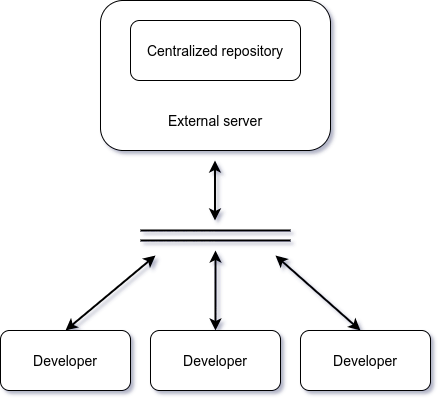
\includegraphics[height=0.6\textheight]{000-vcs-centralized.png}
        \centering
    \end{figure}
\end{frame}

\begin{frame}
    \frametitle{\secname: \small\subsecname\normalsize}

    \begin{columns}
        % Left side
        \column{0.35\textwidth}
            \begin{figure}[h]
                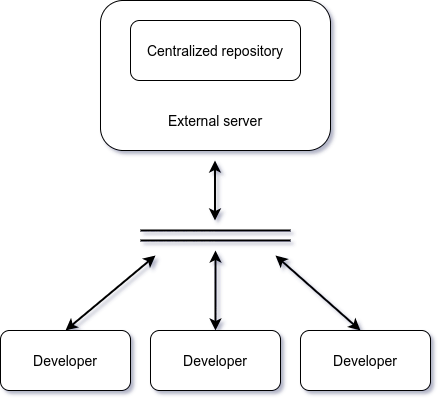
\includegraphics[width=\textwidth]{000-vcs-centralized.png}
                \centering
            \end{figure}

        % Right side
        \column{0.65\textwidth}
            \begin{itemize}
                \item Only the centralizing entity has a copy of the entire repository
                \item Every operation requires communicating with the centralizing entity
                \begin{itemize}
                    \item Checking out a specific version
                    \item Committing new versions
                    \item Checking the history of the repository
                    \item Etc.
                \end{itemize}
            \end{itemize}
    \end{columns}
\end{frame}

%%================================================================================
%%
\subsection{VCS - Distributed VCS}
%%
%%================================================================================
\begin{frame}
    \frametitle{\secname: \small\subsecname\normalsize}

    Everyone has a copy of the entire repository.

    \begin{figure}[h]
        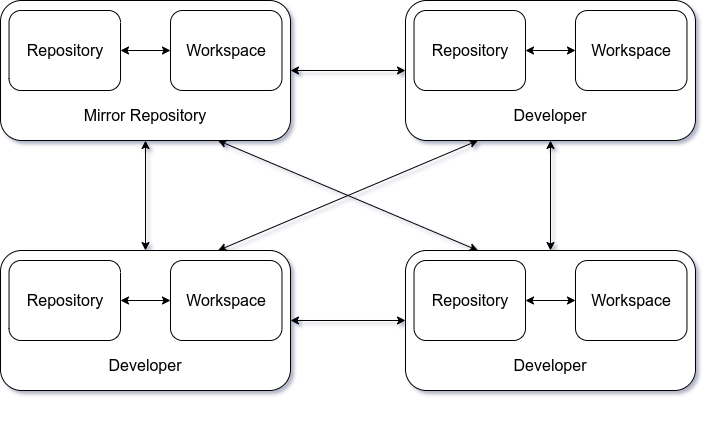
\includegraphics[width=\textwidth]{000-vcs-distributed-plain}
        \centering
    \end{figure}
\end{frame}

\begin{frame}
    \frametitle{\secname: \small\subsecname\normalsize}

    \begin{columns}
        % Left side
        \column{0.35\textwidth}

        \begin{figure}[h]
            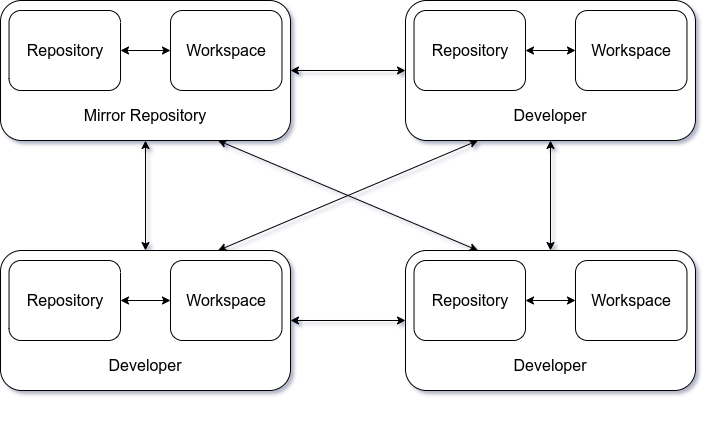
\includegraphics[width=\textwidth]{000-vcs-distributed-plain}
            \centering
        \end{figure}

        % Right side
        \column{0.65\textwidth}
            \begin{itemize}
                \item Most operations may be done in the local repository
                \begin{itemize}
                    \item Checking out a specific (and previously downloaded) version
                    \item Committing new versions
                    \item Checking the (downloaded) history of the repository
                    \item Etc.
                \end{itemize}
                \item New versions may be pushed or retrieve to remote repositories
            \end{itemize}
    \end{columns}
\end{frame}

\begin{frame}
    \frametitle{\secname: \small\subsecname\normalsize}

    One entity (or more) may be selected as the "official" repository

    \begin{figure}[h]
        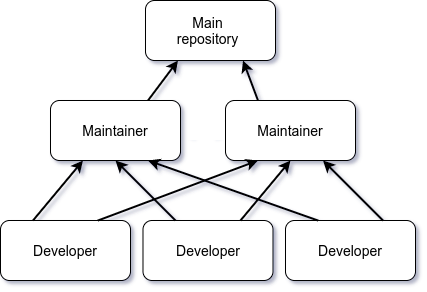
\includegraphics[width=0.75\textwidth]{000-vcs-distributed-hierarchy}
        \centering
    \end{figure}
\end{frame}

\section{What's Git?}

%%================================================================================
%%
\subsection{How does Git work?}
%%
%%================================================================================

\begin{frame}
    \frametitle{\secname: \small\subsecname\normalsize}

    \begin{itemize}
        \item Distributed VCS
        \item Initially made as Linux's VCS, to handle and manage large repositories
        \begin{itemize}
            \item In version 5.13 there were:
            \begin{itemize}
                \item 16,306 new commits
                \item ~800,000 lines changed
                \item Involvement of more than 2,000 developers
            \end{itemize}
        \end{itemize}
        \item Each commit represent a new version of the project
        \item A version is a snapshot of the entire repository
    \end{itemize}

    Losing information is really hard! (more on this later)
\end{frame}

%%================================================================================
%%
\subsection{Naming versions}
%%
%%================================================================================

\begin{frame}
    \frametitle{\secname: \small\subsecname\normalsize}

    When you commit a new version to your local repository, Git assigns an identifier to it.

    % git log --decorate=short --decorate-refs-exclude='refs/remotes/*' --decorate-refs-exclude='refs/tags/*' --date-order  --graph --abbrev-commit  --date=short --pretty='format:%C(auto)%d %h (%cd) %s'
    \begin{figure}[h]
        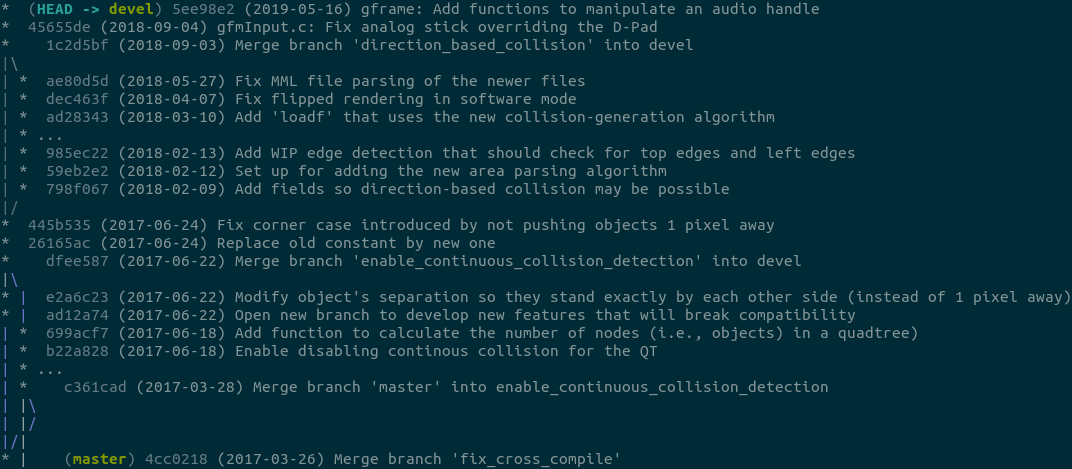
\includegraphics[width=\textwidth]{001-git-commits-example}
        \centering
    \end{figure}
\end{frame}

%%================================================================================
%%
\subsection{Identifying versions}
%%
%%================================================================================

\begin{frame}
    \frametitle{\secname: \small\subsecname\normalsize}

    There are two options to easily track these identifiers:

    \begin{columns}
        % Left side
        \column{0.35\textwidth}

        \begin{figure}[h]
            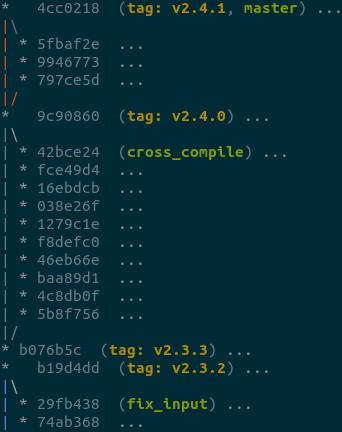
\includegraphics[width=\textwidth]{001-git-branches-example}
            \centering
        \end{figure}

        % Right side
        \column{0.65\textwidth}

        % git log --decorate=short --decorate-refs-exclude='refs/remotes/*' --date-order  --graph --abbrev-commit  --date=short --pretty='format:%C(auto)%h %d ...' master
        \begin{itemize}
            \item \textbf{Tags}: An immutable references to a specific version
            \item \textbf{Branches}: A mutable reference to a version
        \end{itemize}
    \end{columns}

    % XXX: \\ Can't be used as there's no line before this one to be ended
    % (since the last command was a 'column' context).
    \vspace{\baselineskip}
    In both cases, the reference should be meaningfully identified!
\end{frame}

\begin{frame}
    \frametitle{\secname: \small\subsecname\normalsize}

    \textit{HEAD} is a special reference used by Git to identify what's currently checked out in the workspace.

    \begin{figure}[h]
        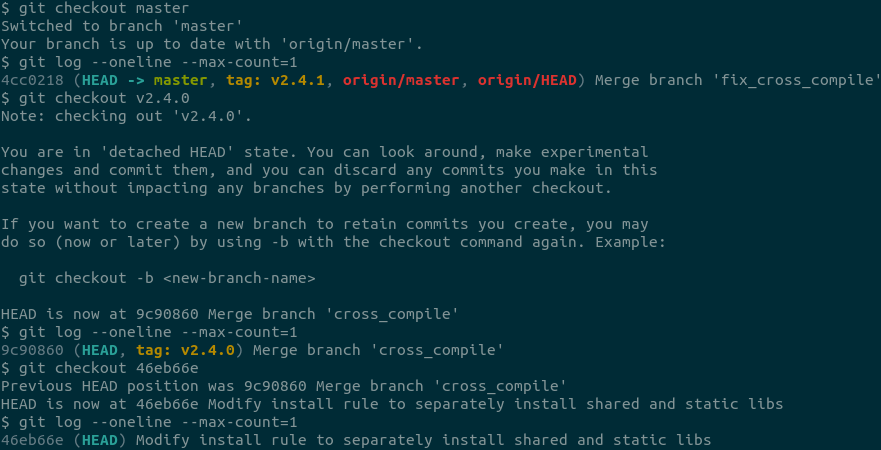
\includegraphics[width=0.8\textwidth]{001-git-checkout-example}
        \centering
    \end{figure}

    \begin{alertblock}{NOTE}
        If Git says something like \textit{You are in 'detached HEAD' state.}, then \textit{HEAD} isn't referencing any branch at all!
    \end{alertblock}
\end{frame}

%%================================================================================
%%
\subsection{"Public" infrastructure vs "Private" infrastructure}
%%
%%================================================================================

\begin{frame}
    \frametitle{\secname: \small\subsecname\normalsize}

    From my personal experience:

    \begin{itemize}
        \item \textbf{Public project}: Changes are made to private copies and later merged back into the original repository
        \item \textbf{Private project}: Changes are made directly to a unique remote copy of the repository
    \end{itemize}

    \begin{columns}
        % Left side
        \column{0.5\textwidth}
        \begin{figure}[h]
            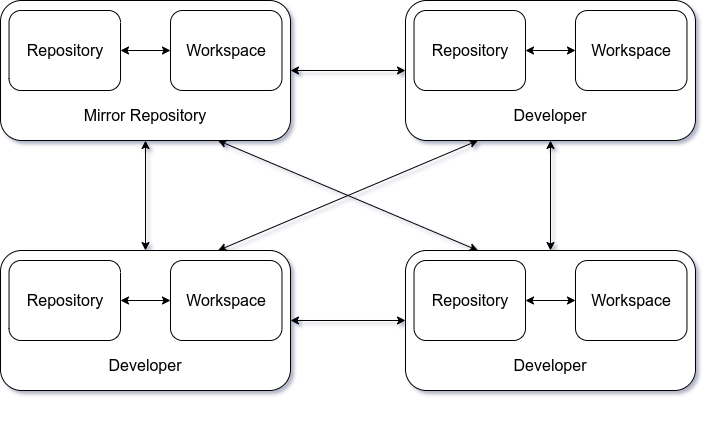
\includegraphics[width=0.95\textwidth]{000-vcs-distributed-plain}
            \centering
        \end{figure}

        % Right side
        \column{0.5\textwidth}
        \begin{figure}[h]
            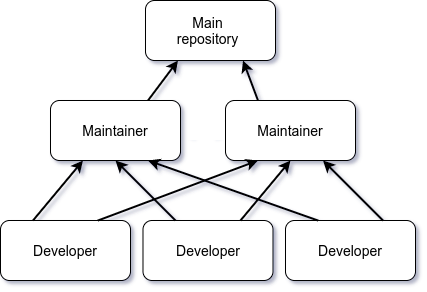
\includegraphics[width=0.95\textwidth]{000-vcs-distributed-hierarchy}
            \centering
        \end{figure}
    \end{columns}
\end{frame}

\begin{frame}
    \frametitle{\secname: \small\subsecname\normalsize}

    Public project example: Linux kernel

    \textit{BASE\_URL}: \small https://git.kernel.org/pub/scm/linux/kernel/git/ \normalsize

    \begin{columns}
        % Left side
        \column{0.35\textwidth}
        \begin{figure}[h]
            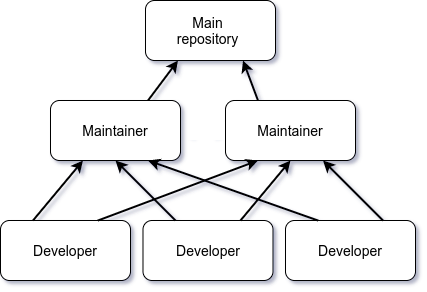
\includegraphics[width=0.95\textwidth]{000-vcs-distributed-hierarchy}
            \centering
        \end{figure}

        % Right side
        \column{0.65\textwidth}
        \begin{itemize}
            \item \textbf{Main repo}: Linus Torvalds' Linux repository
            \begin{itemize}
                \item \small \textit{BASE\_URL}/torvalds/linux.git \normalsize
            \end{itemize}
            \item \textbf{Maintainer}: Staging driver subsystem:
            \begin{itemize}
                \item \small \textit{BASE\_URL}/gregkh/staging.git \normalsize
            \end{itemize}
            \item \textbf{Maintainer}: Media subsystem:
            \begin{itemize}
                \item \small \textit{BASE\_URL}/mchehab/linux-media.git \normalsize
            \end{itemize}
            \item Etc.
        \end{itemize}
    \end{columns}
\end{frame}

%%================================================================================
%%
\subsection{Repository's state}\label{repo-state}
%%
%%================================================================================

\begin{frame}
    \frametitle{\secname: \small\subsecname\normalsize}

    A Git project has three main sections:

    \begin{itemize}
        \item \textbf{Git directory}: Your local copy of the entire repository
        \begin{itemize}
            \item Downloaded when you \textit{clone} a repository from any remote source
        \end{itemize}
        \item \textbf{Working tree}: A single \textit{checkout} of one version of the project, taken from the Git directory
        \begin{itemize}
            \item Basically, everything tracked by Git in the \textit{workspace}
            \item There may be files in the \textit{workspace} that Git isn't tracking
            \item A \textit{bare} copy of a repository is a copy without the \textit{Working tree}
        \end{itemize}
        \item \textbf{Staging area}: changes are marked to go into your next commit
        \begin{itemize}
            \item Stored in the \textit{Git directory}
            \item Relevant enough to deserve its own mention
        \end{itemize}
    \end{itemize}
\end{frame}

\begin{frame}
    \frametitle{\secname: \small\subsecname\normalsize}

    Files in your workspace may be in one of two states:

    \begin{itemize}
        \item \textbf{Tracked}: The file was in the last snapshot, or was staged to be added to the next snapshot
        \item \textbf{Untracked}: The file wasn't in the last snapshot
    \end{itemize}

    Git can't display changes in \textit{untracked}  files since, as far as Git is concerned, those files are brand new.
\end{frame}

\begin{frame}
    \frametitle{\secname: \small\subsecname\normalsize}

    Git has three main states that your files can reside in:

    \begin{itemize}
        \item \textbf{Modified}: The file has changes, either when compared to the latest commit or to the Staging area
        \item \textbf{Staged}: This specific version of the file is marked to be part of the next version
        \item \textbf{Committed}: The data is safely stored in the Git directory
        \begin{itemize}
            \item Could also be called \textit{Unmodified}
        \end{itemize}
    \end{itemize}

    \begin{alertblock}{NOTE}
        These states are exclusively related to the local repository! They don't mean anything in regards to the remote repository!
    \end{alertblock}
\end{frame}

\begin{frame}
    \frametitle{\secname: \small\subsecname\normalsize}

    A file may be both \textit{Modified} and \textit{Staged}, if it was modified after being staged (or if it was only partially staged).

    \begin{figure}[h]
        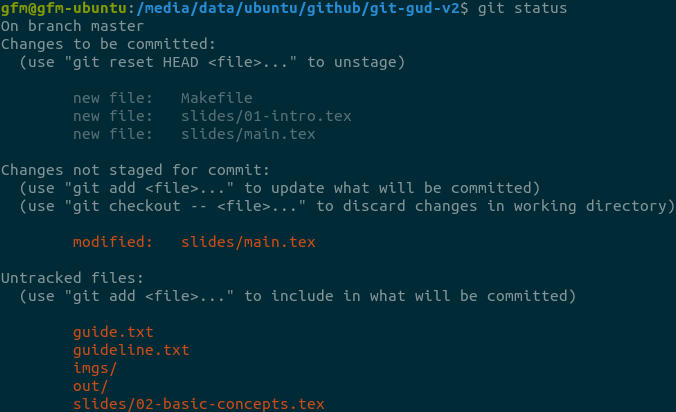
\includegraphics[width=0.9\textwidth]{001-git-areas}
        \centering
    \end{figure}
\end{frame}

%%================================================================================
%%
\subsection{Making changes}
%%
%%================================================================================

\begin{frame}
    \frametitle{\secname: \small\subsecname\normalsize}

    Git creates a snapshot of the entire repository when it creates a new version (commit).

    However, it's OK to think of commits as "changes since the last commit".

    \begin{figure}[h]
        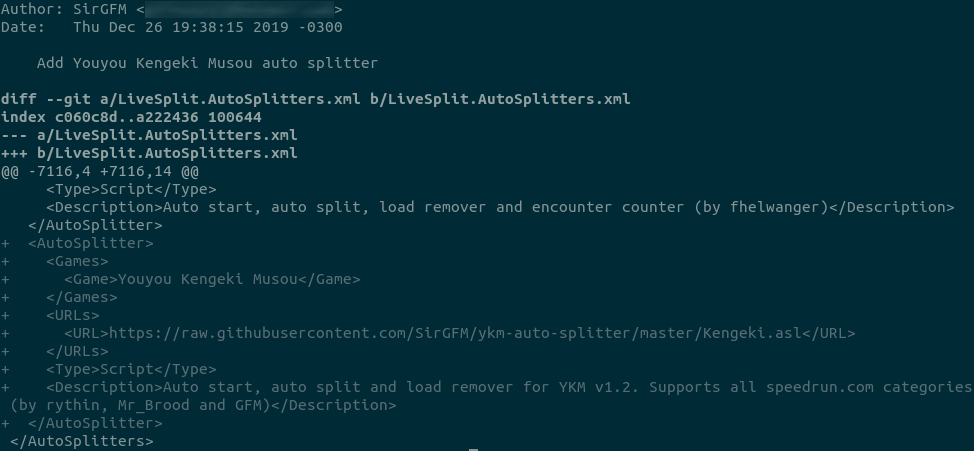
\includegraphics[width=0.95\textwidth]{001-git-diff}
        \centering
    \end{figure}
\end{frame}

%%================================================================================
%%
\subsection{Remote repositories}
%%
%%================================================================================

\begin{frame}
    \frametitle{\secname: \small\subsecname\normalsize}

    Although most operations are done locally, Git is also able to interact with external repositories, called \textit{Remotes}.

    \begin{columns}
        % Left side
        \column{0.5\textwidth}
        \begin{figure}[h]
            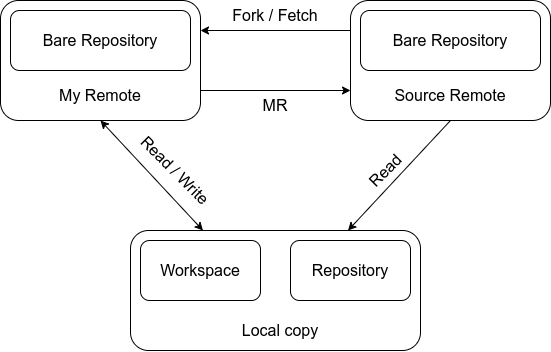
\includegraphics[width=0.95\textwidth]{001-git-remote}
            \centering
        \end{figure}

        % Right side
        \column{0.5\textwidth}
        \begin{figure}[h]
            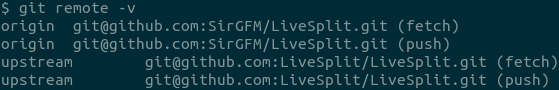
\includegraphics[width=0.95\textwidth]{001-git-remote-example}
            \centering
        \end{figure}
    \end{columns}
\end{frame}

%%================================================================================
%%
\subsection{Integrating changes}
%%
%%================================================================================

\begin{frame}
    \frametitle{\secname: \small\subsecname\normalsize}

    Git repository management services provide means to request that changes made to a given repository/branch are merged into another repository/branch.

    \begin{itemize}
        \item \textbf{Github}: Pull Request
        \item \textbf{Gitlab}: Merge Request
    \end{itemize}

    \begin{figure}[h]
        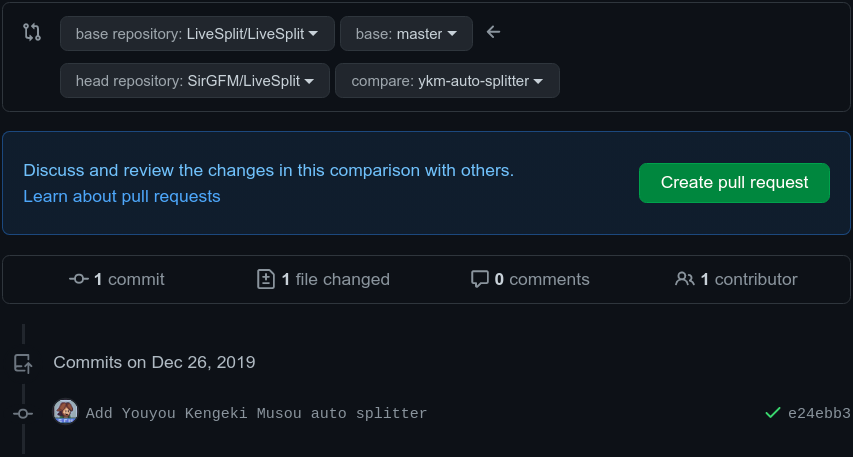
\includegraphics[width=0.8\textwidth]{001-github-mr}
        \centering
    \end{figure}
\end{frame}

\begin{frame}
    \frametitle{\secname: \small\subsecname\normalsize}

    What about repositories outside of one of these services? \\~\\

    For example, how are changes merged back into the Linux kernel?

    \begin{itemize}
        \item Thousands of repositories
        \item Repositories stored in various services/domains
        \item Even local/"offline" repositories
    \end{itemize}
\end{frame}

\begin{frame}
    \frametitle{\secname: \small\subsecname\normalsize}

    \begin{figure}[h]
        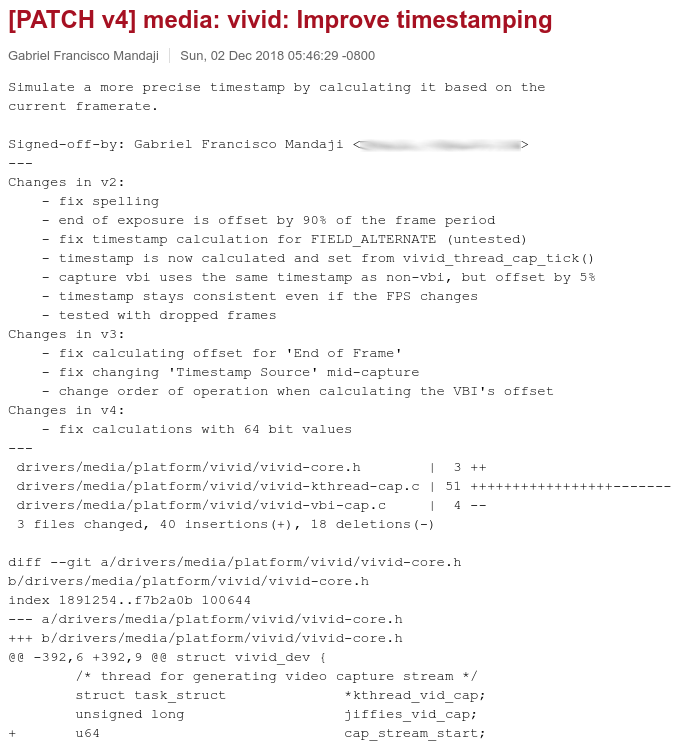
\includegraphics[height=0.8\textheight]{001-linux-mr}
        \centering
    \end{figure}

    Answer: e-mail
\end{frame}

\section{How to use (overview)}

%%================================================================================
%%
\subsection{Basic commands}
%%
%%================================================================================

% XXX: Use the following to take screenshots
% export PS1='\[\e]0;git-talk: \w\a\]${debian_chroot:+($debian_chroot)}\[\033[01;32m\]git-talk\[\033[00m\]:\[\033[01;34m\]\w\[\033[00m\]\$ '

\begin{frame}
    \frametitle{\secname: \small\subsecname\normalsize}

    \begin{itemize}
        \item \texttt{git init}: Create a git repository
        \begin{itemize}
            \item \texttt{git init --bare}: Create a bare git repository
        \end{itemize}
        \item \texttt{git status}: Display the status of local branch
        \item \texttt{git add <file> ...}: Stage something to be committed
        \begin{itemize}
            \item \texttt{git add -p <file> ...}: Interactively stage changes
            \item \texttt{git add -e <file> ...}: Manually edit the changes to be staged
        \end{itemize}
        \item \texttt{git rm <file> ...}: Stage the deletion of a file
        \item \texttt{git reset [HEAD] <file> ...}: Unstage something
        \begin{itemize}
            \item \texttt{git reset -p [HEAD] <file> ...}: Interactively unstage changes
        \end{itemize}
    \end{itemize}
\end{frame}

\begin{frame}
    \frametitle{\secname: \small\subsecname\normalsize}

    \begin{itemize}
        \item \texttt{git commit}: Commit a new version with the staged changes
        \begin{itemize}
            \item \texttt{git commit -m '...'}: Commit with the given message (instead of opening a text editor)
            \item \texttt{git commit -v}: Show the staged changes on the editor
            \item \texttt{EDITOR=vim git commit}: Edit the commit message on VIM
            \item \texttt{git commit --amend}: Commit the staged changes to the last commit (can also be used to edit the commit message)
        \end{itemize}
        \item \texttt{git diff <ref>}: Check changes from \textit{ref} to \textit{HEAD}
        \begin{itemize}
            \item \texttt{git diff -R <ref>}: Invert the diff (i.e., from \textit{HEAD} to \textit{ref})
            \item \texttt{git diff <ref1> <ref2>}: Check the changes between two versions
        \end{itemize}
    \end{itemize}
\end{frame}

%%================================================================================
%%
\subsection{Repository management}
%%
%%================================================================================

\begin{frame}
    \frametitle{\secname: \small\subsecname\normalsize}

    \begin{itemize}
        \item \texttt{git status}: Display the status of local branch
        \begin{itemize}
            \item See section \nameref{repo-state}
        \end{itemize}
        \item \texttt{git branch}: List the local branches
        \begin{itemize}
            \item \texttt{git branch -a}: List all known local and remote branches
            \item \texttt{git branch <name>}: Create a new branch at HEAD
            \item \texttt{git branch <name> <ref>}: Create a new branch at \textit{ref}
            \item \texttt{git branch -d <name>}: Delete the branch
        \end{itemize}
        \item \texttt{git tag <name>}: Create a new tag at HEAD
        \begin{itemize}
            \item \texttt{git tag -m '...' <name>}: Create an annotated tag
        \end{itemize}
    \end{itemize}
\end{frame}

\begin{frame}
    \frametitle{\secname: \small\subsecname\normalsize}

    \begin{itemize}
        \item \texttt{git checkout}: Move things from the \textit{Git Repository} to the \textit{Workspace}
        \begin{itemize}
            \item \texttt{git checkout <ref>}: Check out \textit{ref} (a branch/tag/commit)
            \item \texttt{git checkout <file>}: Discard changes in the file
            \begin{itemize}
                \item Can be understood as "check out the stored version of \textit{file}"
            \end{itemize}
            \item \texttt{git checkout <ref> <file>}: Check out \textit{file} from \textit{ref}
            \item \texttt{git checkout -b <ref>}: Create branch \textit{ref} and check it out
        \end{itemize}
    \end{itemize}

    \begin{alertblock}{NOTE}
        None of these commands alter the \textit{Staging area}!
    \end{alertblock}
\end{frame}


\begin{frame}
    \frametitle{\secname: \small\subsecname\normalsize}

    \begin{itemize}
        \item \texttt{git reset <ref>}: Keep the workspace, but reset the current branch back to \textit{ref}
        \begin{itemize}
            \item \texttt{git reset --hard <ref>}: \textbf{Discard} the workspace and reset the current branch
        \end{itemize}
    \end{itemize}
\end{frame}

%%================================================================================
%%
\subsection{Remote management}
%%
%%================================================================================

\begin{frame}
    \frametitle{\secname: \small\subsecname\normalsize}

    \begin{itemize}
        \item \texttt{git remote [-v]}: List the remote repositories
        \begin{itemize}
            \item \texttt{git remote add <name> <url>}: Add a remote pointing to \textit{url} referenced as \textit{name}
        \end{itemize}
        \item \texttt{git fetch [<ref>]}: Update remote references on the \textit{Git repository}
        \begin{itemize}
        \item \texttt{git fetch [<ref>]}: Update remote references on the \textit{Git repository}
            \item \textit{ref} defaults to \textit{origin} (or to the local branch's remote)
            \item Local branches aren't affected!
        \end{itemize}
        \item \texttt{git push}: Send the local commits to the remote repository
    \end{itemize}
\end{frame}

%%================================================================================
%%
\subsection{Integrating changes}
%%
%%================================================================================

\begin{frame}
    \frametitle{\secname: \small\subsecname\normalsize}

    \begin{itemize}
        \item \texttt{git merge <ref>}: Merge \textit{ref} into \textit{HEAD}
        \begin{itemize}
            \item \texttt{git merge --ff <ref>}: If possible, simply updates \textit{HEAD} to point to \textit{ref} (the default behaviour)
            \item \texttt{git merge --no-ff <ref>}: Force the creation of a merge commit
        \end{itemize}
        \item \texttt{git pull [<ref>]}: Shortcut for \textit{git fetch} followed by \textit{git merge}
    \end{itemize}
\end{frame}

\begin{frame}
    \frametitle{\secname: \small\subsecname\normalsize}

    \texttt{git rebase --onto=<newbase> <base>}: Move all commits between \textit{base} and \textit{HEAD} to \textit{newbase}

    \begin{figure}[h]
        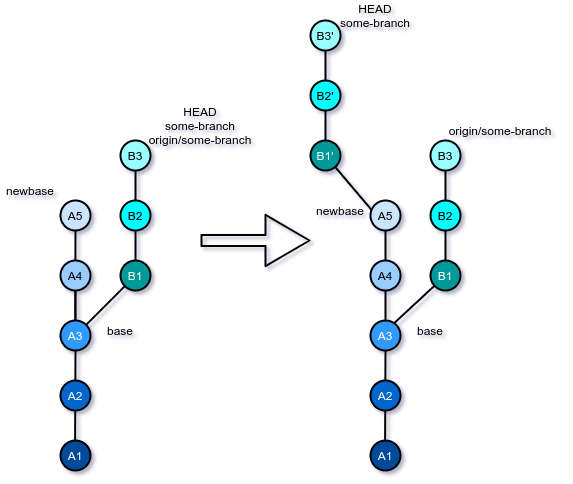
\includegraphics[height=0.65\textheight]{004-rebase}
        \centering
    \end{figure}
\end{frame}

\begin{frame}
    \frametitle{\secname: \small\subsecname\normalsize}

    \begin{itemize}
        \item \textit{Rebase} should be used to move a set of changes from a point to another
        \item Keeps the history clean
        \begin{itemize}
            \item No merge commit except on the main branch
            \item MR only has changes related to that specific MR
            \begin{itemize}
                \item Observed by running \texttt{git diff <base-commit>}
            \end{itemize}
        \end{itemize}
        \item \textbf{Cannot \texttt{git pull} after a rebase!}
        \item Must \texttt{git push --force-with-lease} after rebasing
        \item \texttt{git rebase -i --onto=<newbase> <base>}
        \begin{itemize}
            \item \texttt{-i} stands for "interactive"
        \end{itemize}
    \end{itemize}
\end{frame}

\section{Demo}

\begin{frame}
    \frametitle{\secname}

    Time to demonstrate how to actually use the commands!
\end{frame}


\end{document}
